
\begin{figure*}[!t]
%\vspace{.3in}
\centering
\begin{subfigure}[b]{0.33\textwidth}
  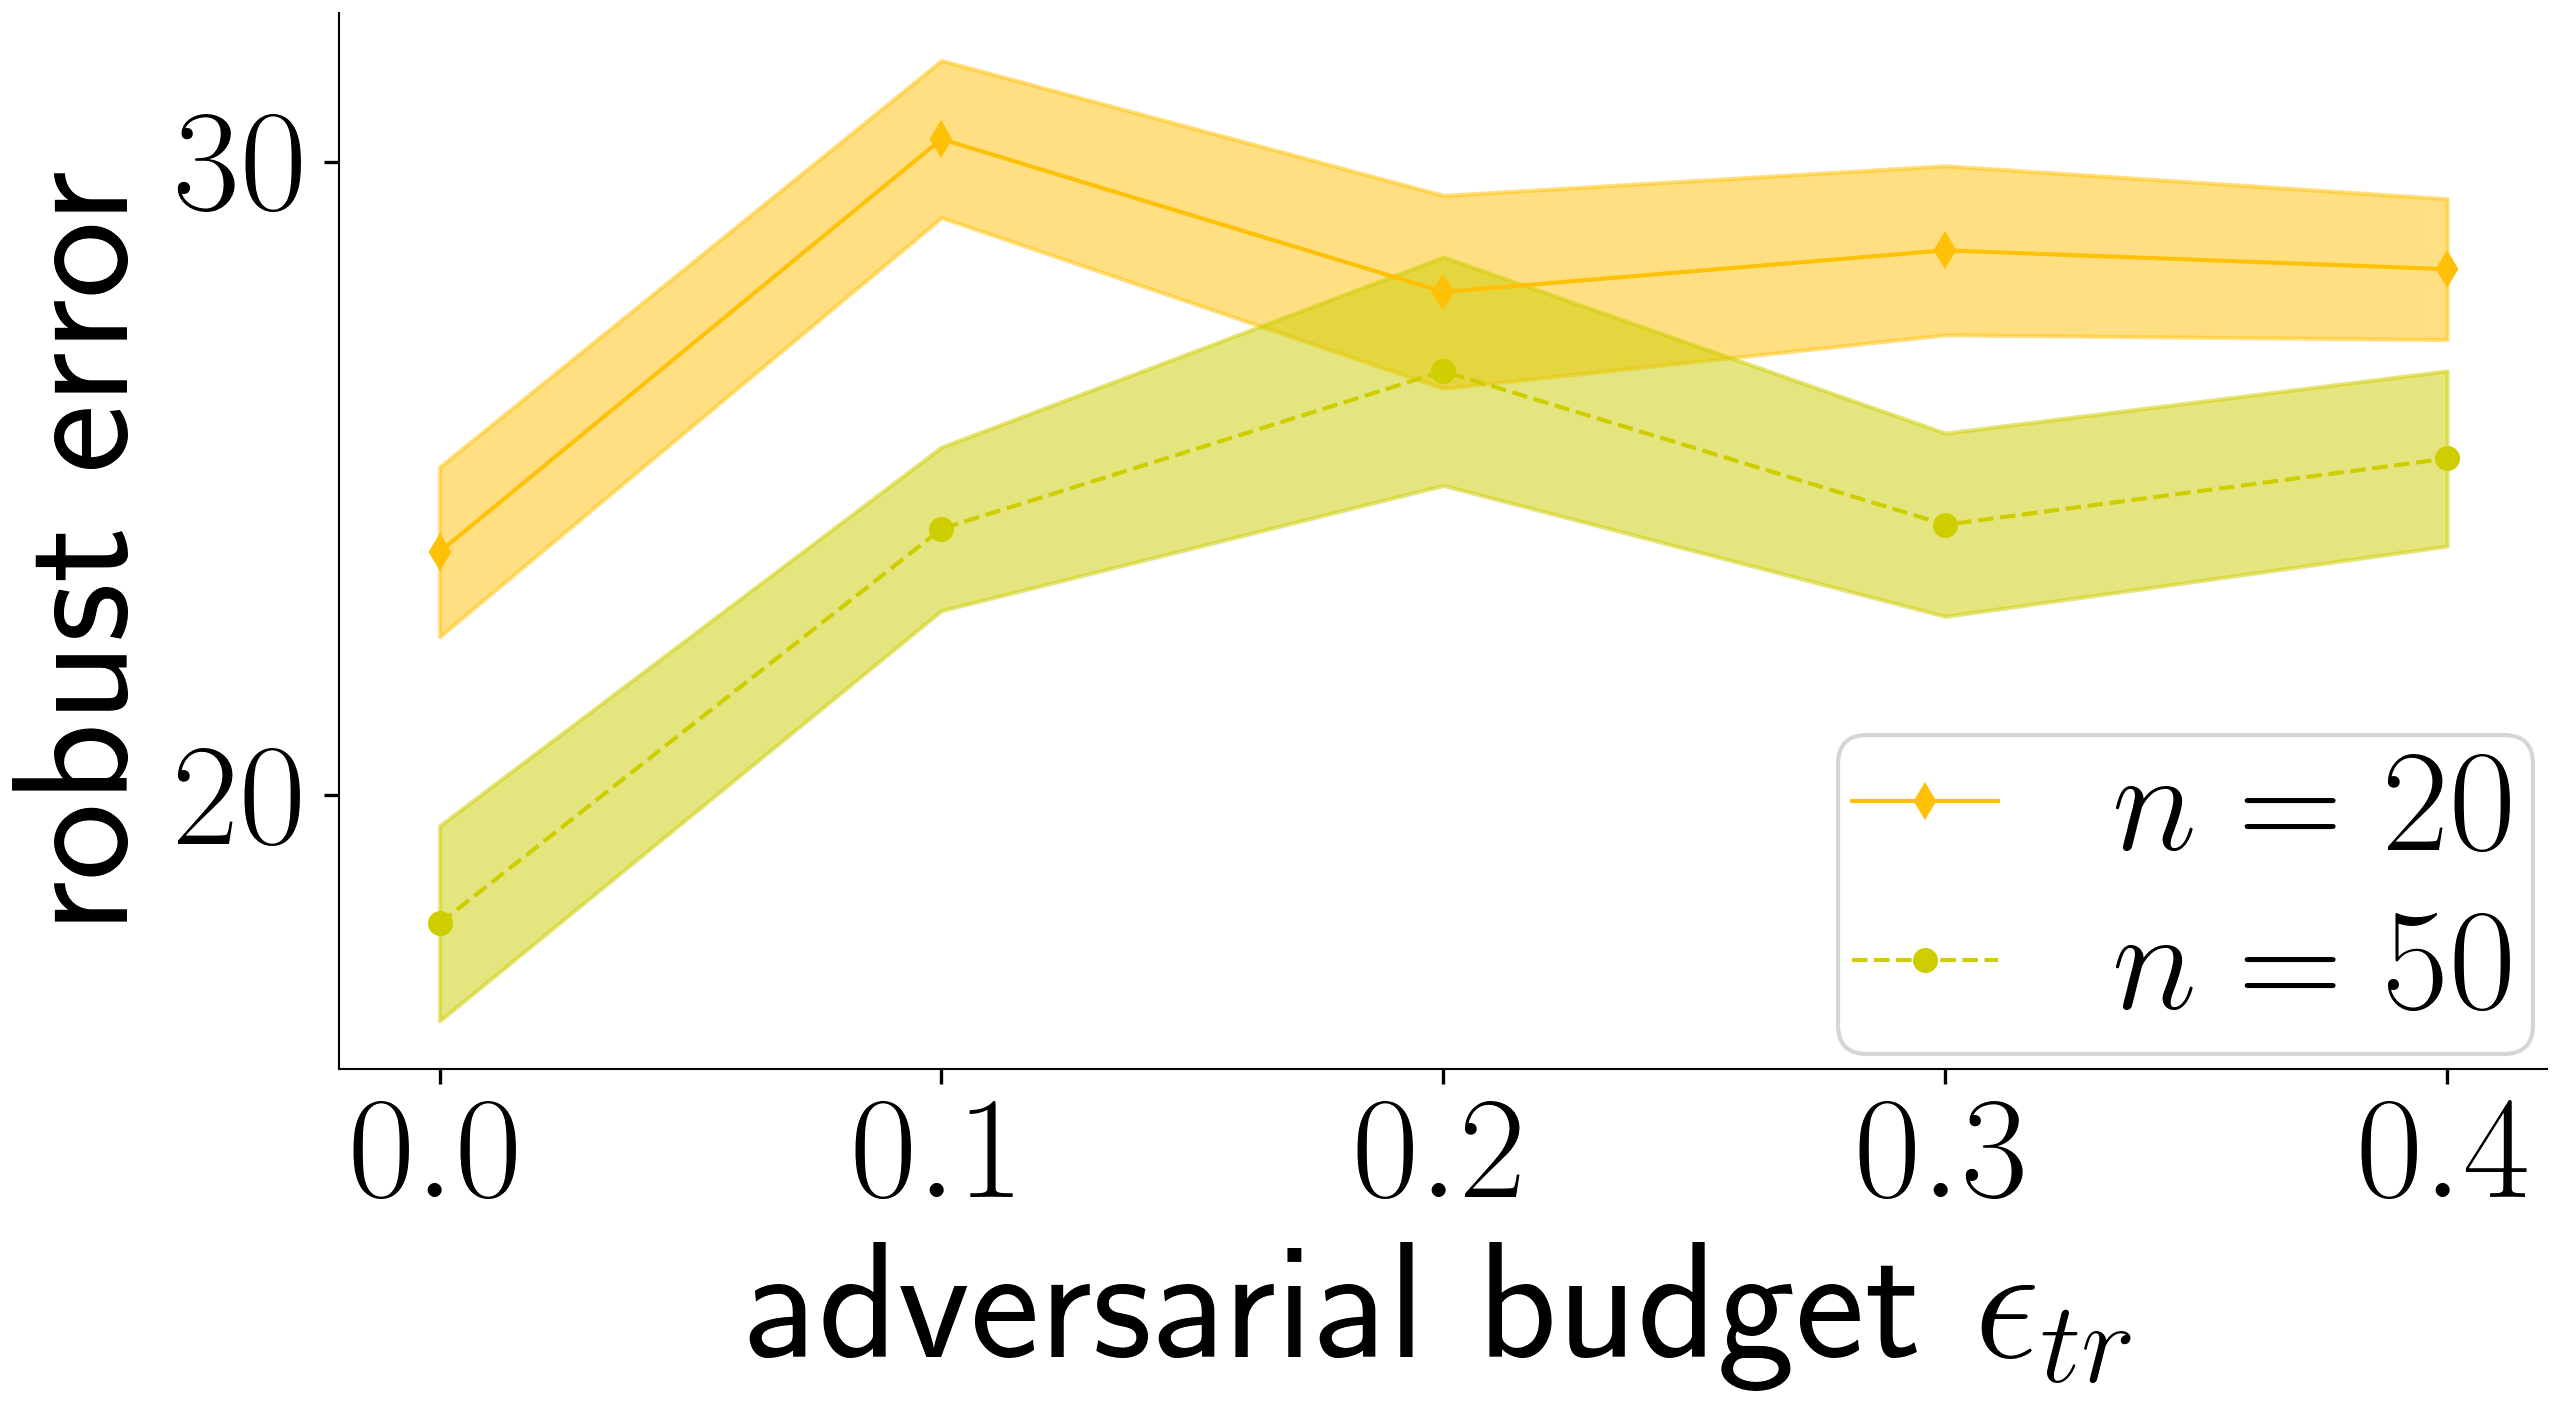
\includegraphics[width=0.99\linewidth]{plotsAistats/d_n_waterbirds_light.png}
  \caption{Robust error vs $\epstrain$}
  \label{fig:waterbirds_light_d_n}
\end{subfigure}
\begin{subfigure}[b]{0.32\textwidth}
  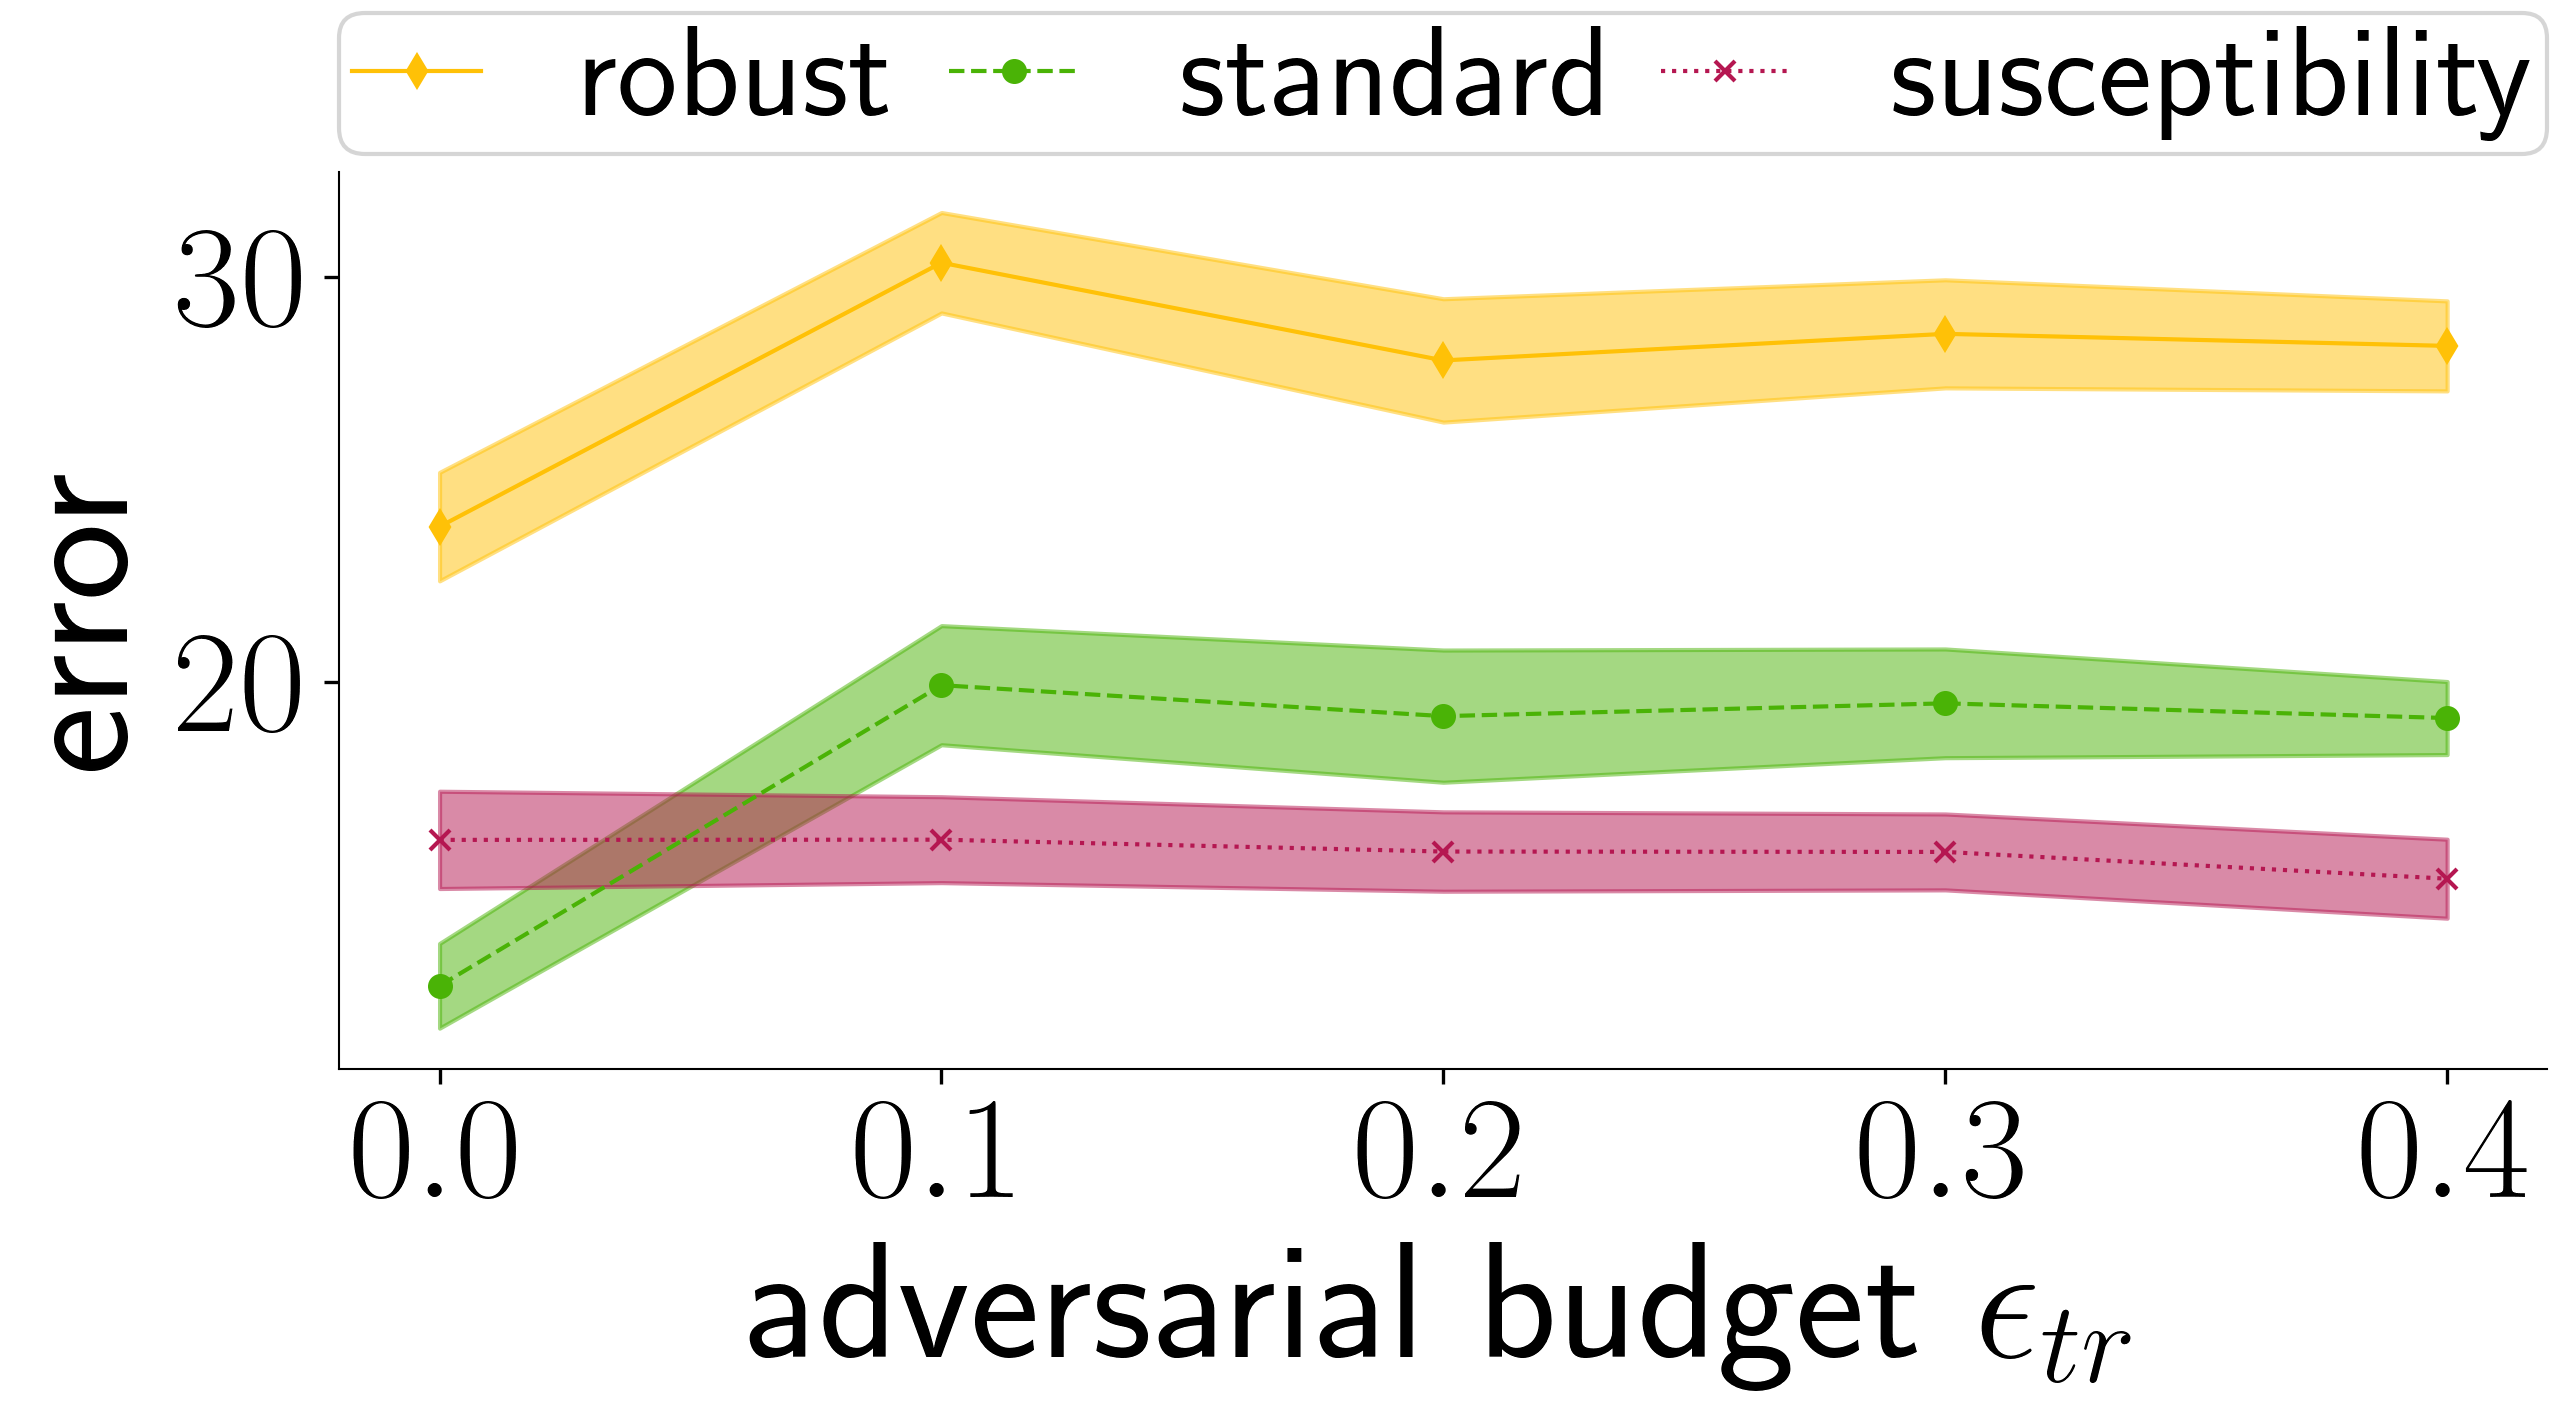
\includegraphics[width=0.99\linewidth]{plotsAistats/waterbirds_light_decomposition.png}
  \caption{Robust error decomposition}
  \label{fig:light_trade_off}
\end{subfigure}
\begin{subfigure}[b]{0.33\textwidth}
  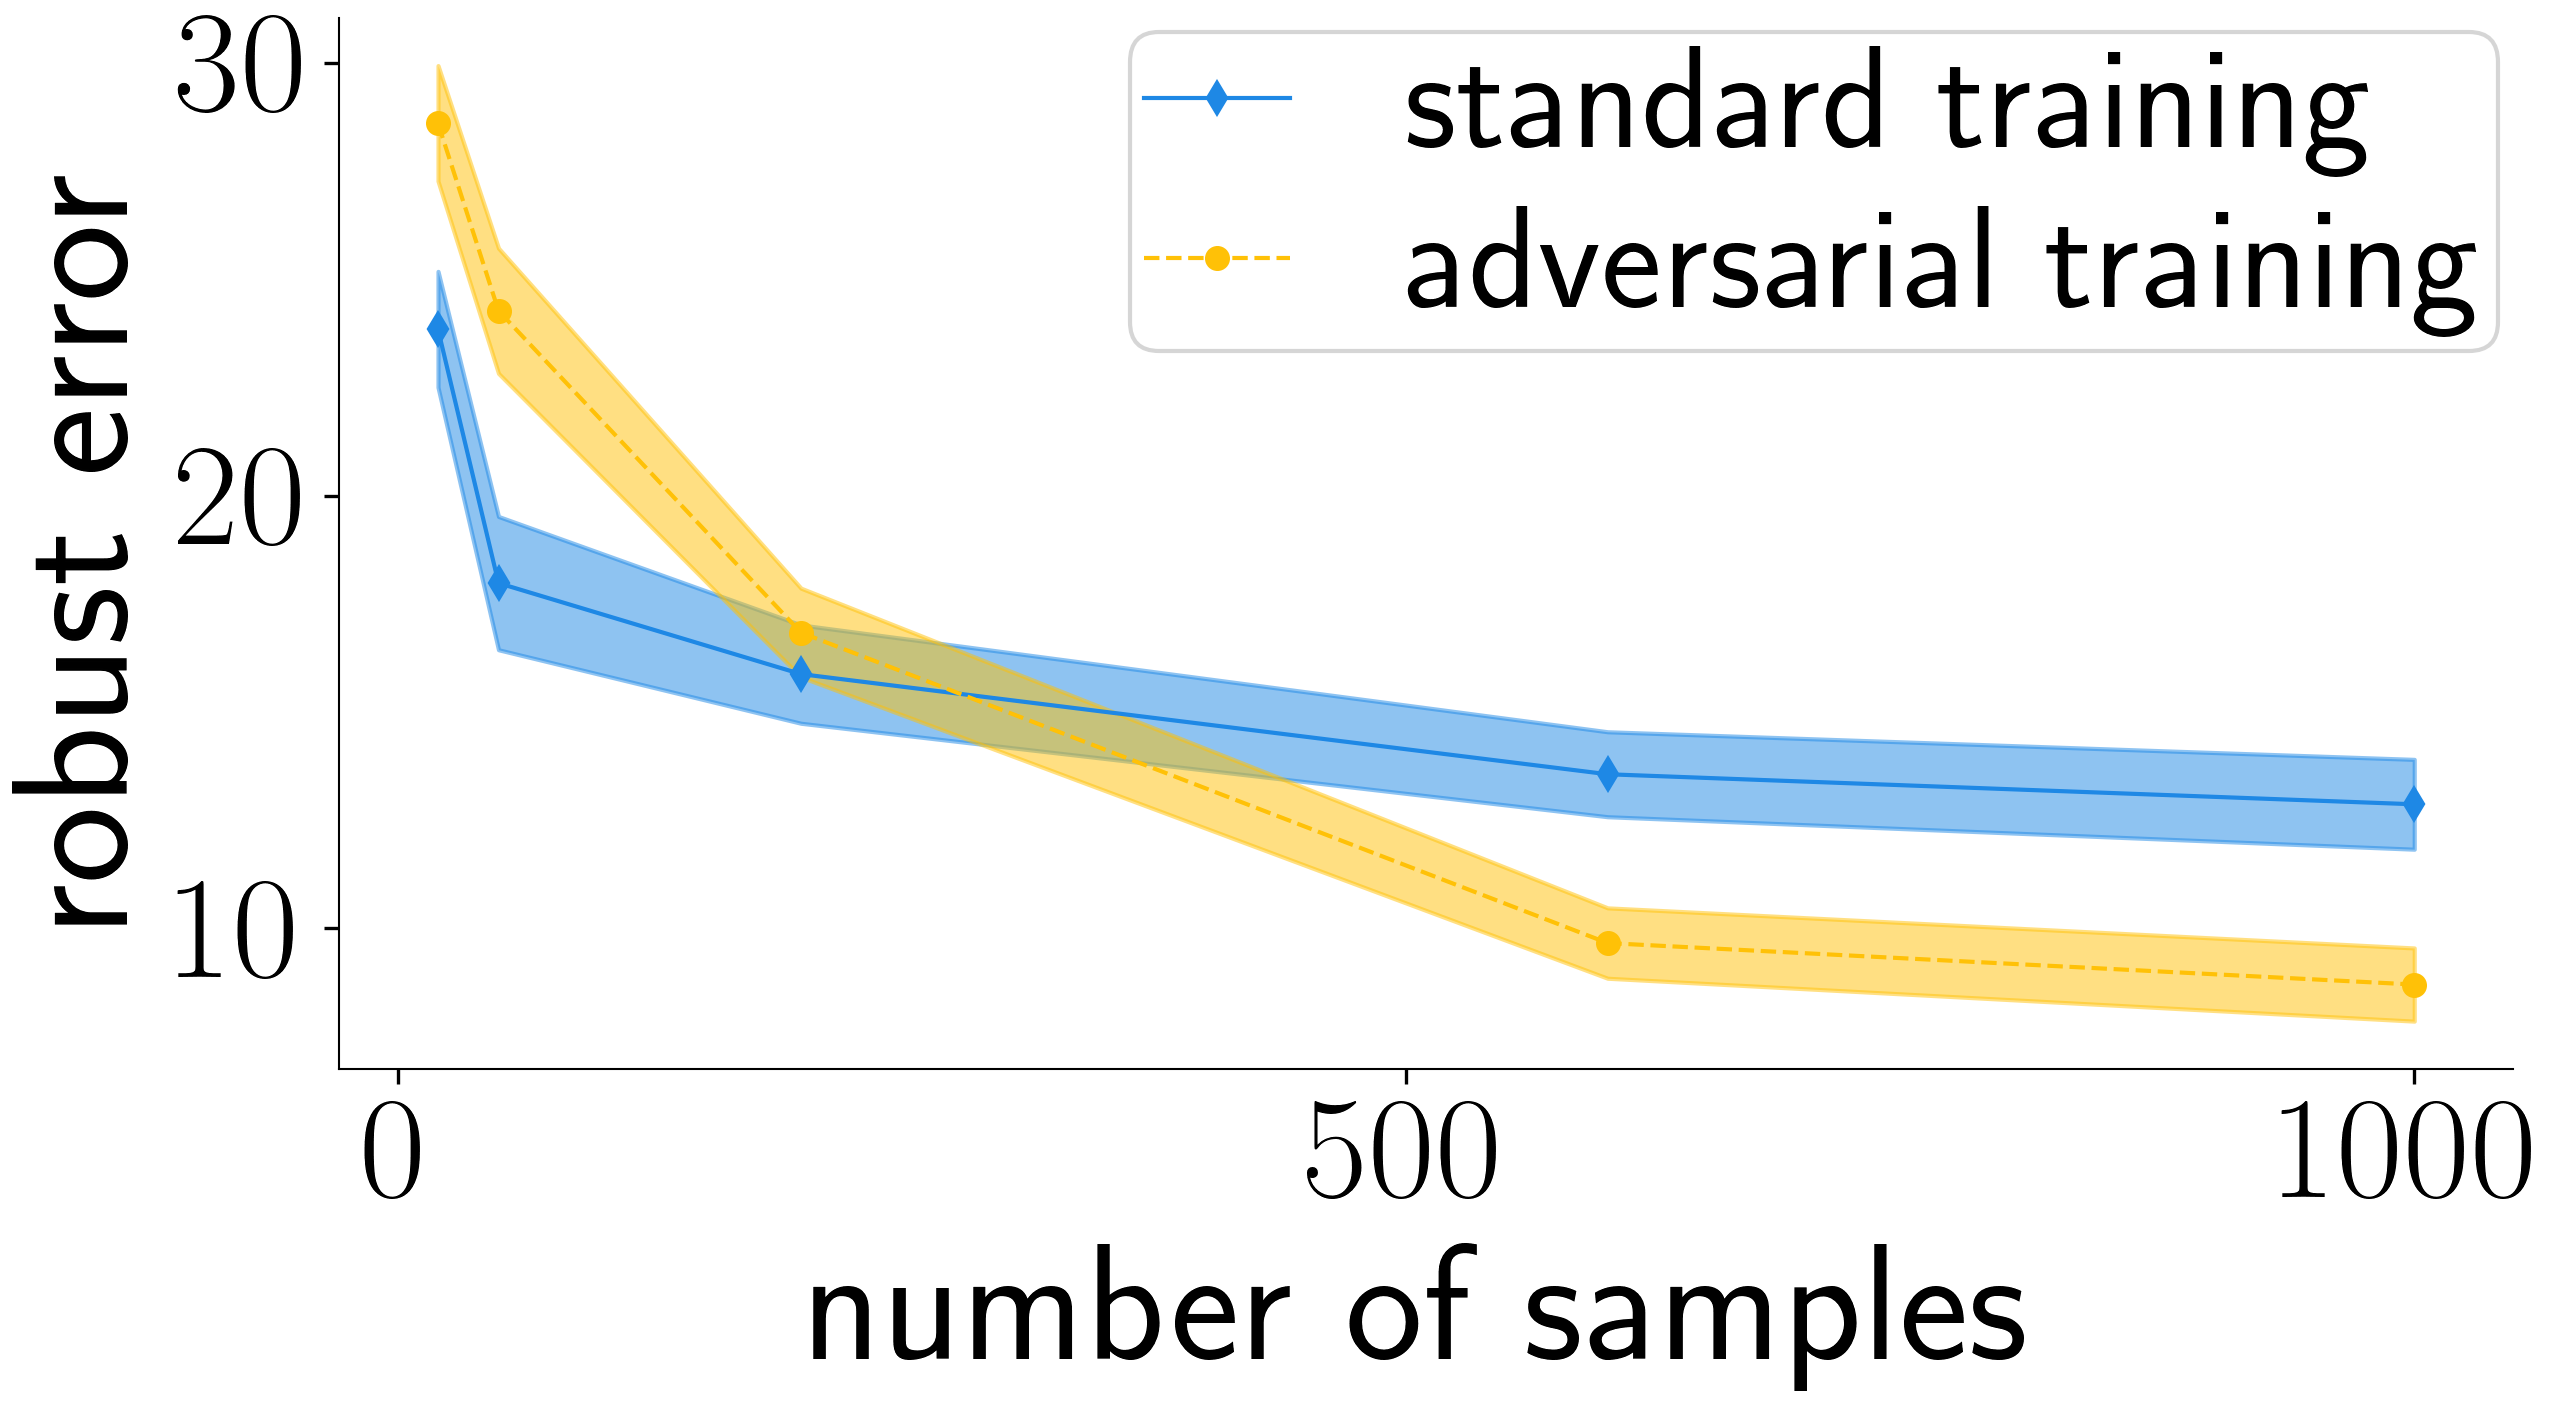
\includegraphics[width=0.99\linewidth]{plotsAistats/numsamp_waterbirds_light.png}
  \caption{Number of samples}
  \label{fig:waterbirds_light_numobs}
\end{subfigure}
  \caption{Experiments on the Waterbirds dataset considering the adversarial illumination attack with $\epstest = 0.3$. We plot the mean and standard deviation of the mean of several independent experiments. (a) The robust error increases with larger $\epstrain$ in the low sample size regime. (b) We set $\numsamp=20$ and plot the robust error decomposition as in Equation $\eqref{eq:decomposition}$ with increasing $\epstrain$. While the susceptibility decreases slightly, the increase in standard error is much more severe, resulting in an increase in robust error. (c) Adversarial training hurts robust generalization in the low sample size regime $(\numsamp < 200)$, but helps when enough samples are available. For more experimental details see Section \ref{sec:waterbirds}.}
\label{fig:waterbirds_light}
%\vspace{.3in}
\end{figure*}

\section{Real-world experiments}
\label{sec:realworldexpapp}

In this section, we demonstrate that adversarial training may
hurt robust accuracy in a variety of image attack scenarios
on the Waterbirds and CIFAR10 dataset.
The corresponding experimental details and more experimental results (including
on an additional hand gestures dataset) can be found in Appendices
 \ref{sec:waterbirds}, \ref{sec:app_cifar10} and \ref{sec:handgestures}.

%% We perform experiments on the Waterbirds dataset, CIFAR10, and a
%% static hand-gesture recognition dataset.
%% %dataset provided by \cite{Mantecon19}. 
%% In this section, we discuss a subset of the experiments, but the
%% complete set of experimental results with extensive experimental
%% details can be found in Appendices \ref{sec:waterbirds} (Waterbirds),
%% \ref{sec:app_cifar10} (CIFAR10) and \ref{sec:handgestures} (hand
%% gestures dataset).
%% more experiments for the datasets CIFAR10, SVHN, waterbirds dataset and the
%% static hand gesture recognition dataset can be found 

\subsection{Datasets}

We now describe the datasets and models that we use for the
experiments. In all our experiments on CIFAR10, we vary the sample
size by subsampling the dataset and use a ResNet18 \cite{He16} as
model. We always train on the same (randomly subsampled) dataset,
meaning that the variances arise from the random seed of the model and
the randomness in the training algorithm. In Appendix
\ref{sec:app_cifar10}, we complement the results of this section by
reporting the results of similar experiments with different
architectures.


As a second dataset, we build a new version of the Waterbirds
dataset, consisting of images of water- and
landbirds of size $256 \times 256$ and labels that distinguish the
two types of birds. We construct the dataset as follows: First, we
sample equally many water- and landbirds from the CUB-200 dataset
\cite{Welinder10}. Then, we segment the birds and paste them onto a
background that is randomly sampled (without replacement) from the Places-256 dataset \cite{zhou17}.
%% where the aim is to recognise if a given image of a bird depicts a land-or waterbird. More concretely, we build the dataset as follows: First, we randomly sample water-and landbirds from the CUB-200 dataset \cite{Welinder10}. Then, we sample equally many background images from the Places-256 dataset \cite{zhou17}, where we only consider the backgrounds: bamboo forest, broadleaf forest, lake and ocean. Lastly, we segment the birds from their original image and paste them onto a random background image. 
%% The CUB dataset consists of images of $200$ bird
%% species with a segmentation mask to cut out the bird and the Places
%% dataset consists of a multitude of backgrounds such as "forest" and
%% "ocean". The segmentation mask is used to cut out the bird of the
%% original picture, which allows us to simulate perturbations such as
%% motion blur on flying objects. The waterbird dataset is generated by
%% classifying all the waterbird vs. landbird species of the CUB dataset,
%% where the background is changed by copy-pasting the birds on
%% backgrounds of the Places dataset. The resulting size of the images is
%% $256$ by $256$.
%%To ensure independence of background colours and types with the label, we ensure that the bird types and backgrounds are balanced in each dataset. Maybe not needed
For the implementation of the dataset we used the code provided by \citet{Sagawa20}. Also, following the choice of \citet{Sagawa20}, we use as model a ResNet50 that was pretrained on ImageNet and which achieves near perfect standard accuracy.


\subsection{Evaluation of \nameofattacks}

We consider three types of \nameofattacks on our real world datasets:
square masks, motion blur and adversarial illumination. The mask
attack is a model used to simulate sticker-attacks and general
occlusions of objects in images \cite{Eykholt18, Wu20}. On the other
hand, motion blur may arise naturally for example when photographing
fast moving objects with a slow shutter speed. Further, adversarial
illumination may result from adversarial lighting conditions or smart
image corruptions. Next, we describe the attacks in more detail.
%An application for all attacks in the low sample size regime is criminal face detection, where the criminal would likely use a disguise, possibly move fast, and choose poor lighting conditions.

\paragraph{Mask attacks}
On CIFAR10, we consider the square black mask attack: the adversary can set a mask
of size $\epstest \times \epstest$ to zero in the image. To ensure that the mask does not cover the whole signal in the image, we
restrict the size of the masks to be at most $2 \times 2$. Hence, the search space of the attack consists of all possible locations of the masks in the targeted image. For exact robust error evaluation, we perform a full grid search over all possible locations during test time. See Figure \ref{fig:CIFAR10_boat} for an example of a mask attack on CIFAR10.
%% For more details on the approximate
%% attack we refer to Appendix \ref{sec:app_cifar10}. 

\paragraph{Motion blur}
On the Waterbirds dataset we consider two \nameofattacks: motion blur and adversarial illumination. For the motion blur attack,
%the adversary can apply different levels of blur to the birds in the images \fy{this is actually not how i wanted to think about blur - an adversary cannot make the bird move quicker, only the bird itself},
the bird may move at different speeds without changing the background. 
%Hence, the motion blur attack mimics the effect of photographing birds, where the bird moves with possibly different speeds in combination with a suboptimal exposure time of the camera lens.
%Clearly, the fast moving object is the bird and not the background.
The aim is to be robust against all motion blur severity levels up to $\motionblurkernel_{max} = 15$. 
To simulate motion blur, we first segment the birds and then use a filter with a kernel of size $\motionblurkernel$ to apply motion blur on the bird only. Lastly, we paste the blurred bird back onto the background image. We can change the severity level of the motion blur by increasing the kernel size of the filter.
%\fy{on the segmented bird image, before pasting onto background? (not using this precise language)}, 
%where the larger the kernel, the more severe the blur on the bird.
%% Note that the faster the bird moves in comparison to the photographer, the more severe the blur. We can simulate different blur levels by changing the kernel size; the larger the kernel, the more severe the blur on the bird.
See Appendix \ref{sec:waterbirds} for an ablation study and concrete expressions of the motion blur kernel. At test time, we perform a full grid search over all kernel sizes to exactly evaluate the robust error. We refer to Figure \ref{fig:WB_motion_blur} and Section \ref{sec:waterbirds} for examples of our motion blur attack.

\paragraph{Adversarial illumination} As a second attack on the Waterbirds dataset, we consider adversarial illumination. The adversary can darken or brighten the bird without corrupting the background of the image. The attack aims to model images where the object at interest is hidden in shadows or placed against bright light. 
%Moreover, the subtlety of the attack allows the adversary to create images that still seem natural, even though corrupted. 
To compute the adversarial illumination attack, we segment the bird, then darken or brighten the it, by adding a constant $a \in [-\epstest, \epstest]$, before pasting the bird back onto the background image. We find the most adversarial lighting level, i.e. the value of $a$, by equidistantly partitioning the interval $[-\epstest, \epstest]$ in $K$ steps and performing a full list-search over all steps.
%\fy{severities? you don't say how you do it? also mention the segmented bit?} 
%We perform a list search over $K$ possible constants by equidistantly seg levels where the perturbation size is less than $\epstest$. %At test time, we take $65$ steps, whereas at training time we take $33$ steps. 
See Figure \ref{fig:WB_light_dark} and Section \ref{sec:waterbirds} for examples of the adversarial illumination attack.


\subsection{Adversarial training procedure}

For all datasets, we run SGD until convergence on the \emph{robust} cross-entropy
loss~\eqref{eq:emploss}. In each iteration, we search for an adversarial example
and update the weights using a gradient with respect to the resulting
perturbed example \cite{goodfellow15, madry18}.
%\fy{cite madry?}.  
For every experiment, we choose the learning
rate and weight decay parameters that minimize the robust error on a
hold-out dataset. We now describe the implementation of the
adversarial search for the three types of
\nameofattacks. 
% \fy{can put this in appendix} On CIFAR10 and
%waterbirds, we train for $100$ epochs and on SVHN for $160$ epochs.
%Since we are in the small sample size regime, we train until convergence in all the
%experiments. \fy{what do you mean? we can? we should?}

\paragraph{Mask attacks}
Unless specified otherwise, we use an approximate attack similar to
\citet{Wu20} during training time:
%by identifying the $K = 16$
%most promising mask locations with a heuristic as follows.
First, we identify promising mask locations by analyzing the gradient, $\nabla_x \loss(f_\theta(x), y)$, of the cross-entropy loss with respect to the input. Masks that cover part of the image where the gradient is large, are more likely to increase the loss. Hence, we compute the $K$ mask locations $(i, j)$, where $\|\nabla_x \loss(f_\theta(x), y)_{[i:i+2, j:j+2]} \|_1$ is the largest and take using a full list-search the mask that incurs the highest loss.
%\fy{what?} where the gradient of the logits \fy{which logit?} with respect to the inputs has the highest $\ell_1$-norm. \fy{don't get it}
%First, we compute the gradient of the logits of the neural network with respect to the input. Then, we identify the $K$ mask locations where the gradient of the logits has the highest $\ell_1$-norm. Lastly,
%We then search among these locations to find the mask that has the largest loss.
Our intuition from the theory predicts that higher $K$,
and hence a more exact ``defense'', only increases the robust error of
adversarial training, since the mask could then more efficiently cover
important information about the class. We indeed confirm this effect
and provide more details in Section~\ref{sec:app_cifar10}.

\paragraph{Motion blur}
Intuitively the worst attack should be the most severe blur, rendering
a search over a range of severity superfluous.  However, similar to
rotations, this is not necessarily true in practice since the training loss on
neural networks is generally nonconvex. Hence, during training time,
we perform a search over kernels with sizes $2i$ for $i = 1,\dots,
\motionblurkernel_{max}/2$. Note that, at test time, we do an exact search
over all kernels of sizes in $[1, 2, \dots, \motionblurkernel_{max}]$.

\paragraph{Adversarial illumination}
Similar to the motion blur attack, intuitively the worst perturbation
should be the most severe lighting changes; either darkening or
illuminating the object maximally. However, again this is not
necessarily the case, since finding the worst attack is a nonconvex
problem. Therefore, during training and testing we partition the
interval $[-\epstrain, \epstrain]$ in $33$ and $65$ steps
respectively, and perform a full grid-search to find the worst
perturbation.

\subsection{Adversarial training can hurt robust generalization}

Further, we perform the following experiments on the Waterbirds dataset using the motion blur and adversarial illumination attack. We vary the adversarial training  budget $\epstrain$, while keeping the number of samples fixed, and compute the resulting robust error.
We see in Figure \ref{fig:waterbirds_light_d_n} and \ref{fig:motion_lines} that, indeed, adversarial training can hurt robust generalization with increasing perturbation budget $\epstrain$.

Furthermore, to gain intuition as described in Section~\ref{logreg_proof_sketch} and, we also plot the robust error decomposition (Equation~\ref{eq:decomposition}) consisting of the standard error and susceptibility in Figure \ref{fig:light_trade_off} and \ref{fig:motion_blur_trade_off}. Recall that we measure susceptibility as the fraction of data points in the test set for
which the classifier predicts a different class under an adversarial attack.
As in our linear example, we observe an increase in robust error despite a slight drop
in susceptibility, because of the more severe increase in standard error. 
%% Adversarial training typically increases robustness and causes a
%% smaller drop in standard accuracy, thereby raising robust accuracy.
%% In our experiment depicted in Figure~\ref{fig:SVHN_tade_off} we
%% perform adversarial training on a subsampled dataset of SVHN with
%% increasing adversarial budget $\epstrain$.
%% Similar to our theoretical
%% results for the linear case, we find that the increase in robustness
%% due to adversarial training is less than the reduction in standard
%% accuracy by it, leading to a worse robust accuracy for increasing
%% $\epstrain$. 
Similar experiments for the hand gesture dataset can be
found in~\ref{sec:handgestures}. 


\begin{figure*}[!t]
%\vspace{.3in}
\centering
\begin{subfigure}[b]{0.4\textwidth}
  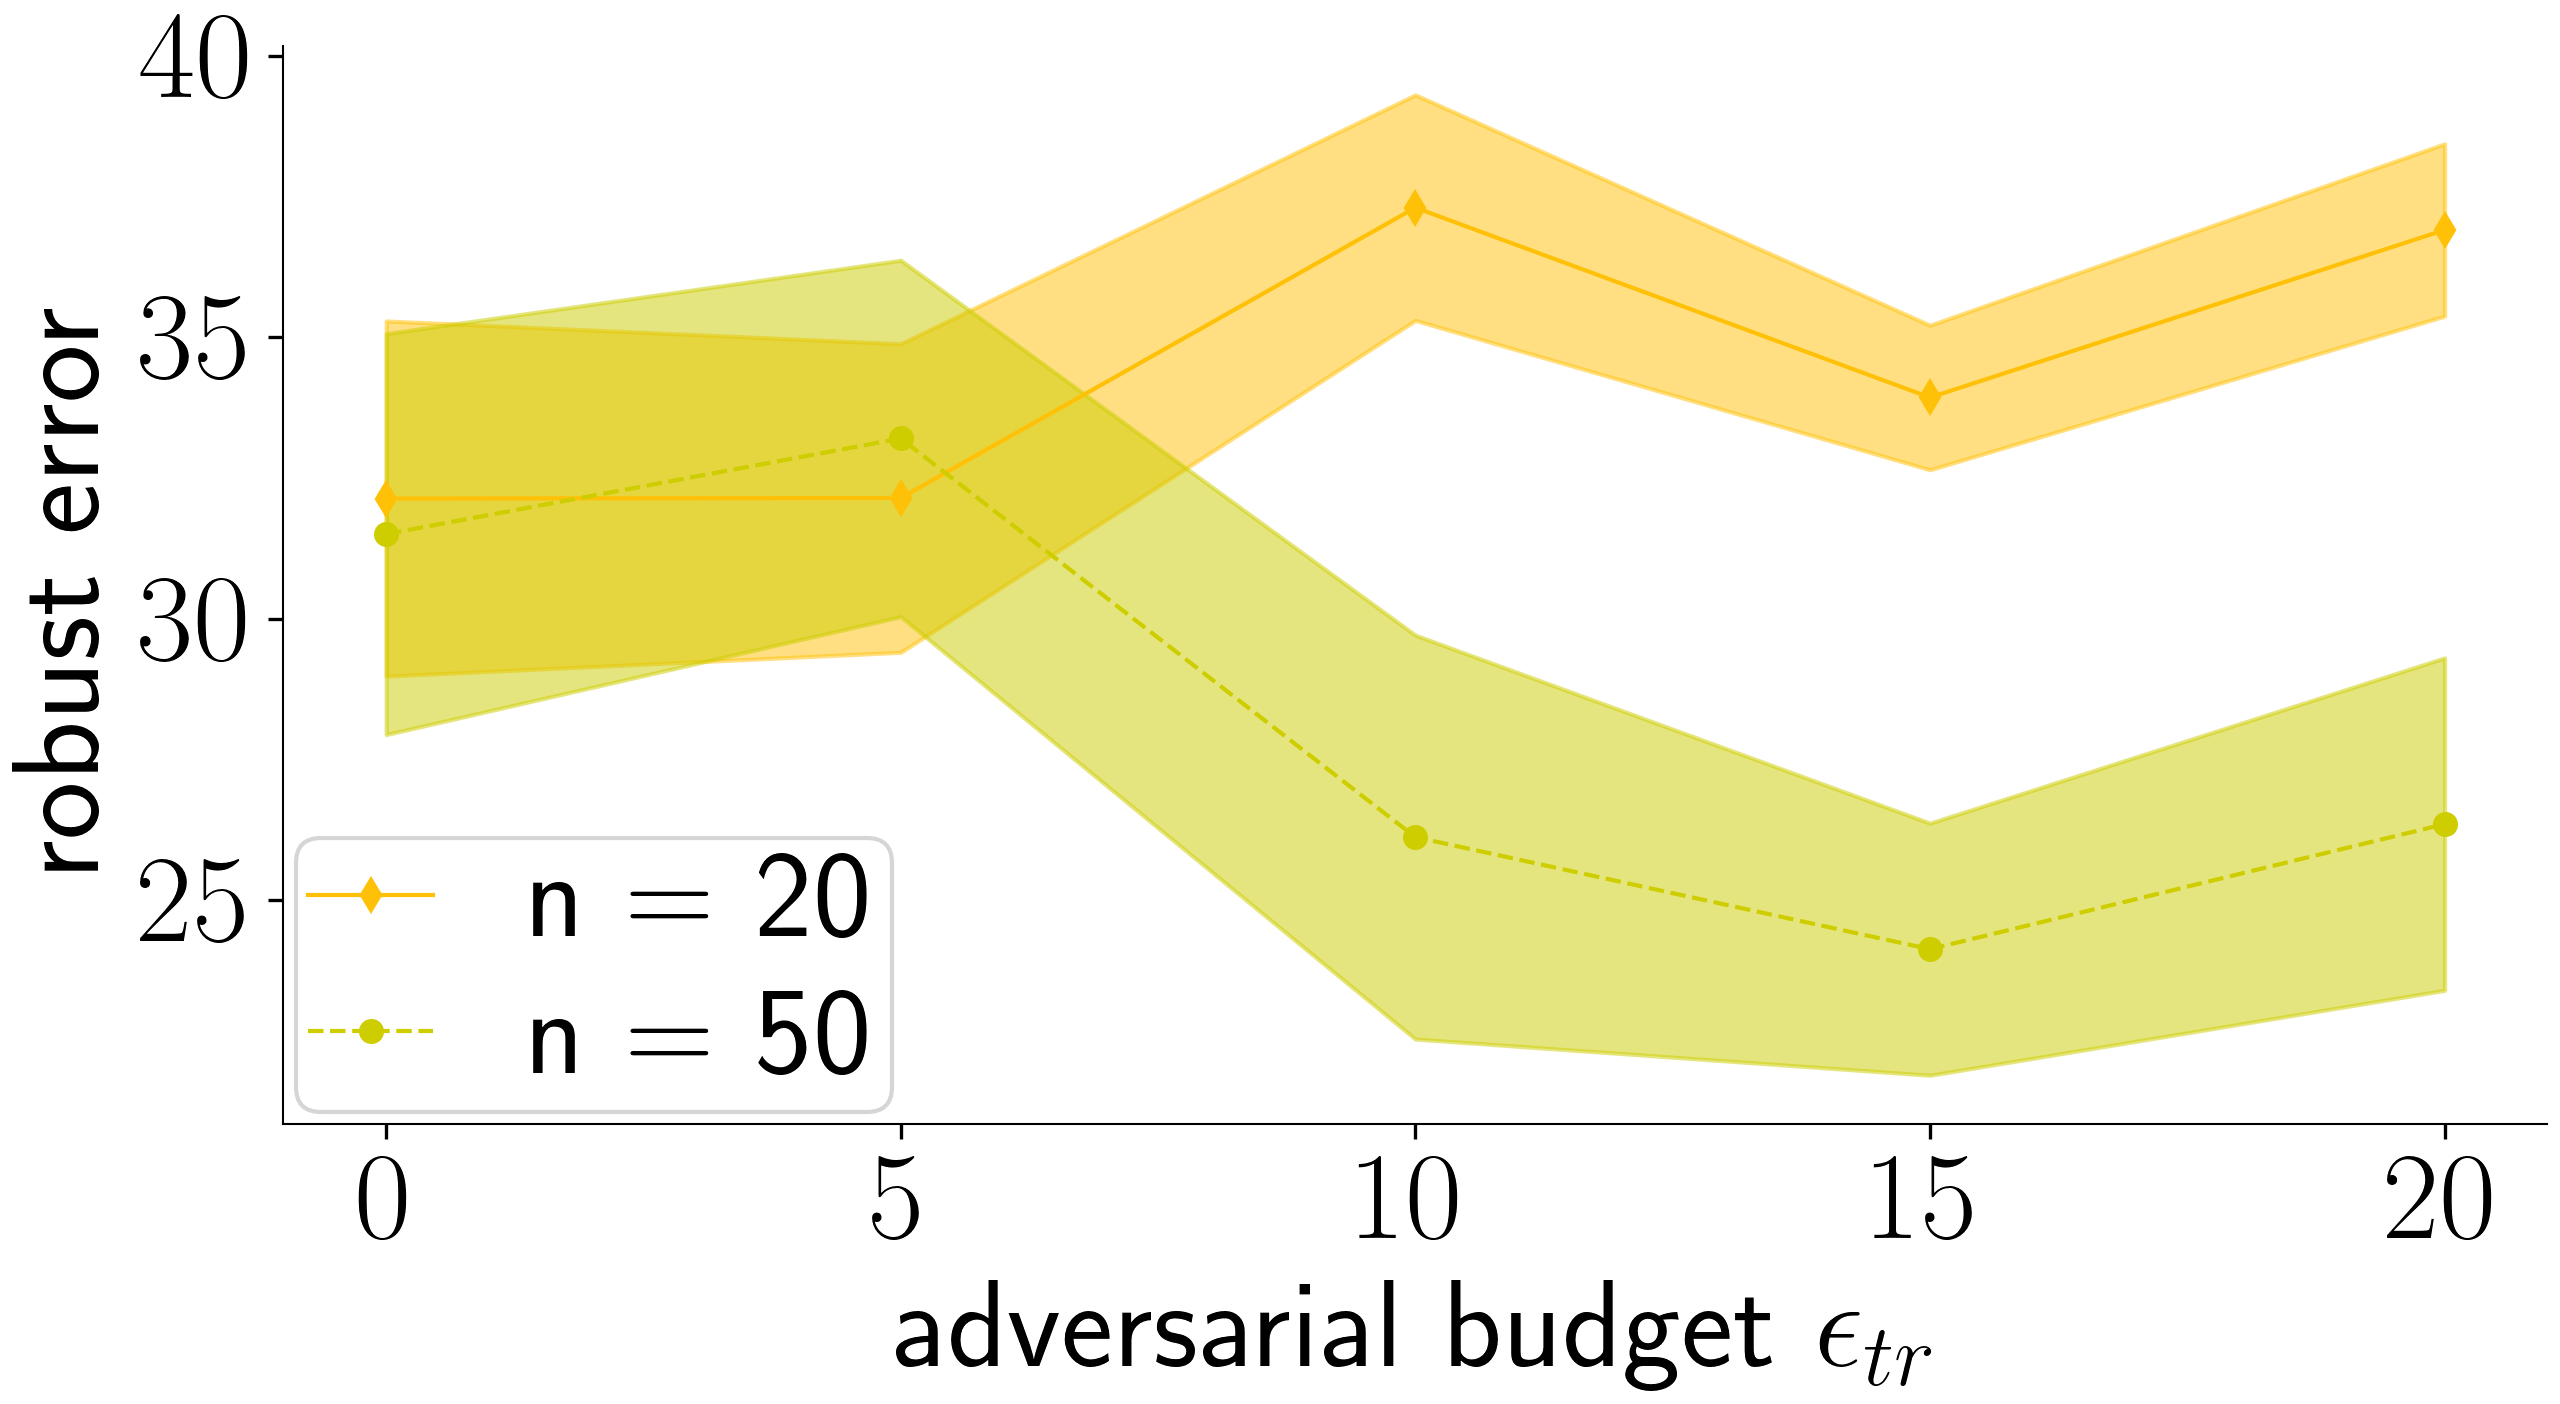
\includegraphics[width=0.99\linewidth]{plotsAistats/waterbirds_motion_d_n.png}
  \caption{Robust error with increasing $\epstrain$}
  \label{fig:motion_lines}
\end{subfigure}
\begin{subfigure}[b]{0.4\textwidth}
  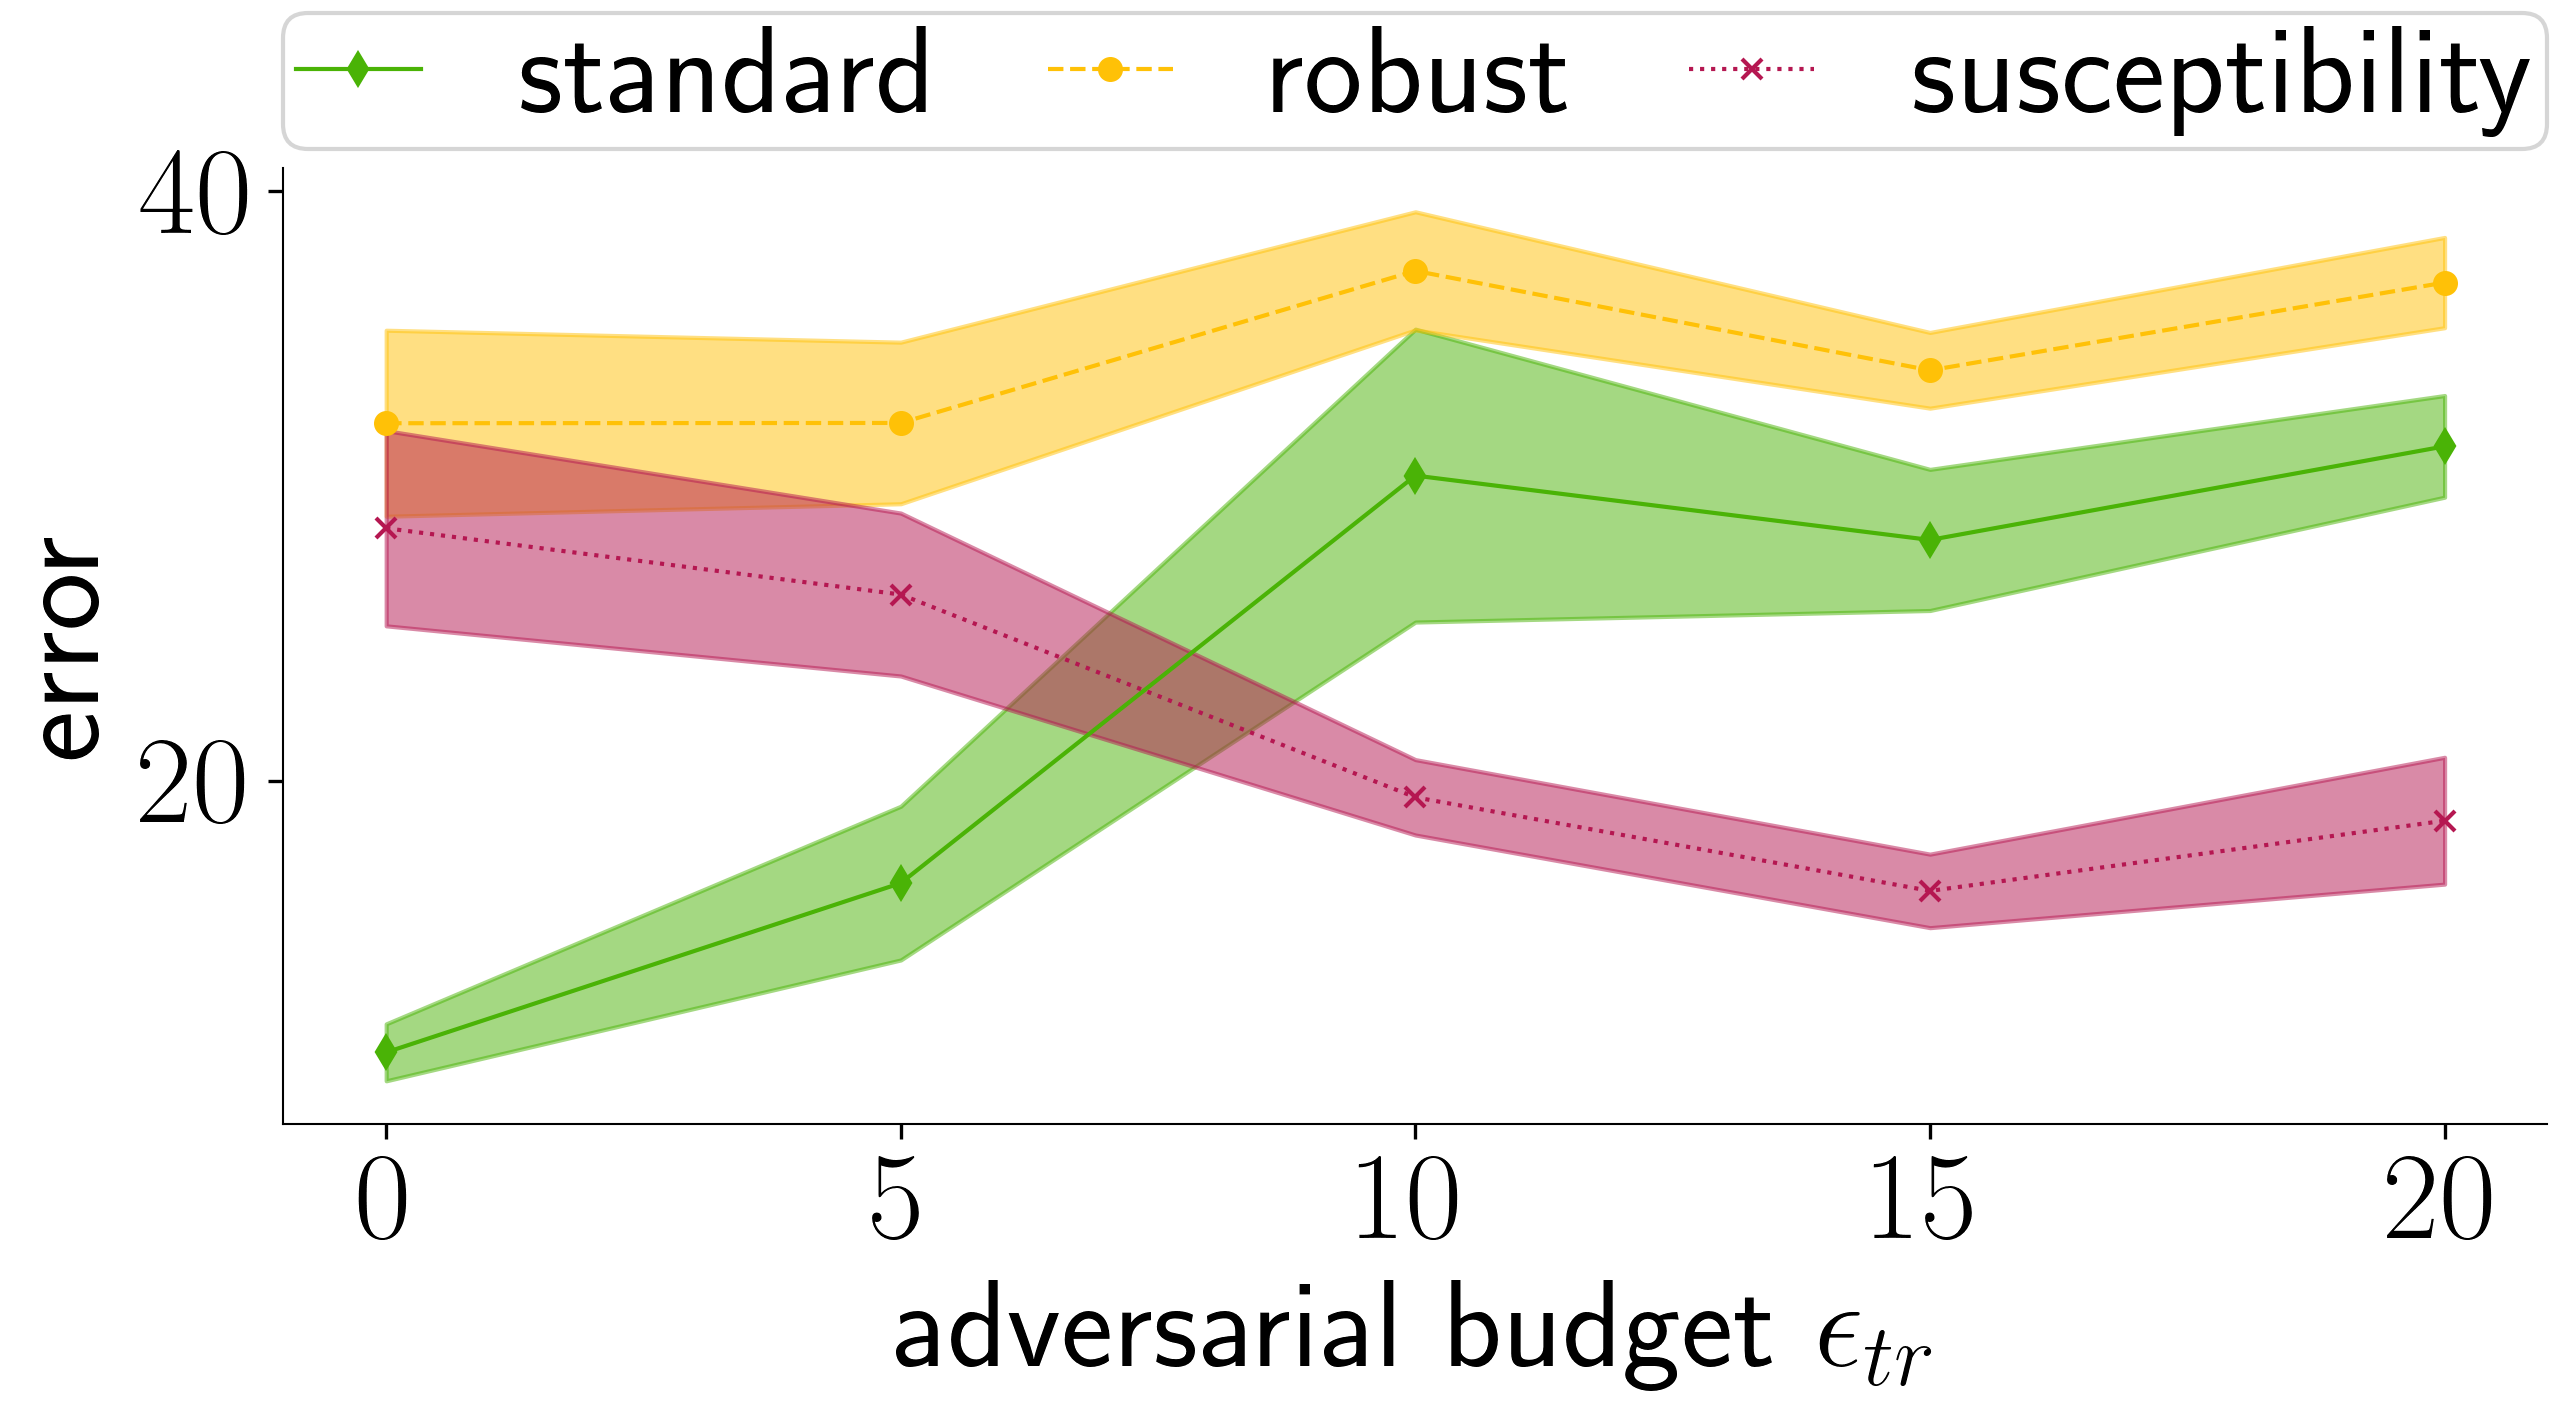
\includegraphics[width=0.99\linewidth]{plotsAistats/waterbirds_trade-off.png}
  \caption{Robust error decomposition}
  \label{fig:motion_blur_trade_off}
\end{subfigure}
  \caption{ (a) We plot the robust error with increasing adversarial training budget $\epstrain$ of $5$ experiments on the subsampled Waterbirds datasets of sample sizes $20$ and $30$. Even though adversarial training hurts robust generalization for low sample size ($\numsamp = 20$), it helps for $\numsamp = 50$.  (b) We plot the decomposition of the robust error in standard error and susceptibility with increasing adversarial budget $\epstrain$. We plot the mean and standard deviation of the mean of $5$ experiments on a subsampled Waterbirds dataset of size $\numsamp = 20$. The increase in standard error is more severe than the drop in susceptibility, leading to a slight increase in robust error. For more experimental details see Section \ref{sec:waterbirds}.}
\label{fig:motion_blur_real_world}
%\vspace{.3in}
\end{figure*}

%% \fy{according to gdoc this should not be here}
%% Furthermore, it is a common belief (see e.g. the discussion on
%% catastrophic overfitting in Section~\ref{sec:relatedwork}) that using
%% the strongest attack (in this case, full grid search) during training
%% should also result in better robust generalization. 
%% %\fy{this figure will go in next section, replaced by svhn masks / waterbird blurs}
%% %\jc{Yes, we'll probably refer to it in appendix due to place constraints}
%% In our experiment depicted in Figure~\ref{fig:K_plot}, we subsample
%% CIFAR10 to a dataset of size $500$ and perform adversarial and
%% standard training. We vary the attack strength $K$ during
%% \emph{training} and find that even though robustness increases, the
%% robust accuracy (when evaluated using full grid search over $K=900$)
%% decreases for increasing attack strength. Full experimental details
%% are provided in Section \ref{sec:app_cifar10}.

%\subsection{Phenomenon inherent to the small sample regime}

%% \fy{refer to teaserplot}
%% Many works already note that adversarial training does raise robust
%% generalization in the high sample regime. Attack-model overfitting is
%% hence a phenomenon inherent to datasets with few samples, as also predicted
%% by our theorem.
As predicted by our theorem, the phenomenon where adversarial training hurts robust generalization is most pronounced in the small sample size regime. Indeed, the experiments depicted in Figures \ref{fig:waterbirds_light_d_n} and \ref{fig:motion_lines} are conducted on small sample size datasets of $\numsamp = 20$ or $50$.
In Figure \ref{fig:teaserplot} and \ref{fig:waterbirds_light_numobs}, we
observe that the as sample size increases,  adversarial training does improve robust generalization compared to standard training, even for \nameofattacks. Moreover, on the experiments of CIFAR10 using the mask perturbation, which can be found in Figure \ref{fig:teaserplot} and Appendix \ref{sec:app_cifar10}, we observe the same behaviour: Adversarial training hurts robust generalization in the low sample size regime, but helps when enough samples are available. 

%% explicitly see
%% that adversarial training does improve robust generalization, even for \nameofattacks, compared to standard training, when the sample size is large enough.
%A detailed comparison of low and small-sample can be found in Appendix \ref{sec:app_cifar10} and Appendix \ref{sec:waterbirds}. Needed?

\subsection{Discussion}

In this section, we discuss how different algorithmic choices, motivated
by related work, affect when and how adversarial training hurts robust generalization. 

\paragraph{Strength of attack and catastrophic overfitting}
In many cases, the worst case perturbation during adversarial training is found using an approximate algorithm such as projected gradient descent. It is common belief  that using the strongest attack (in the mask-perturbation case, full grid search) during training should also result in better robust generalization. 
In particular, the literature on catastrophic overfitting shows that weaker attacks during training lead to bad performance on stronger attacks during testing  \cite{Wong20Fast, andriushchenko20, li21}.
Our result suggests the opposite is true in the low-sample size regime for
\nameofattacks : the weaker the attack, the better
adversarial training performs.
%% We observe this phenomenon depicted in 
%% Figure \ref{fig:K_plot}, where we vary the grid size (and hence attack strength) $K$ during \emph{training}.  Full 
%% experimental details are provided in Section \ref{sec:app_cifar10}.


%% \fy{rephrase} In our theory on the linear models and on the 2-layer
%% neural network, we assume perfect adversarial examples, i.e. we can
%% maximize exactly.  Usually, the more precisely the algorithm finds the
%% maximum (i.e., the stronger the attack) during training, the better
%% the resulting robust test accuracy. Vice versa, weaker attacks during
%% training lead to bad performance on stronger attacks during testing
%% (catastrophic fitting) \cite{Wong20Fast, andriushchenko20, li21}.

%% It
%% is obvious from our theorem that for signal-attacking perturbations,
%% the opposite is true: the better the search, the more likely we find
%% the perturbation that hurts the signal in the sample the most. Hence,
%% the weaker the attack, the better adversarial training performs.  We
%% vary the attack strength $K$ during \emph{training} and find in Figure
%% \ref{fig:K_plot}, that even though robustness increases, the robust
%% accuracy (when evaluated using full grid search over $K=900$)
%% decreases for increasing attack strength. Full experimental details
%% are provided in Section \ref{sec:app_cifar10}.

%% We show the
%% observation experimentally in Figure \ref{fig:K_plot} for the mask
%% attack by changing the grid size $K$ for the location search of the
%% mask \fy{rephrase}. Note that this observation is in fact the opposite
%% statement of the phenomenon called catastrophic overfitting.

%% Furthermore, it is common belief  that using
%% the strongest attack (in this case, full grid search) during training
%% should also result in better robust generalization. 
%% %\fy{this figure will go in next section, replaced by svhn masks / waterbird blurs}
%% %\jc{Yes, we'll probably refer to it in appendix due to place constraints}
%% In our experiment depicted in Figure~\ref{fig:K_plot}, we subsample
%% CIFAR10 to a dataset of size $500$ and perform adversarial and
%% standard training. We vary the attack strength $K$ during
%% \emph{training} and find that even though robustness increases, the
%% robust accuracy (when evaluated using full grid search over $K=900$)
%% decreases for increasing attack strength. Full experimental details
%% are provided in Section \ref{sec:app_cifar10}.

  
%% For example, \cite{Wong20Fast, andriushchenko20, li21} note that performing
%% adversarial training with a one step attack such as the fast gradient
%% sign method (FGSM) \cite{goodfellow15} until convergence may lead to
%% non-robust models against stronger PGD-based attacks during test time,
%% even though it leads to good robust generalization against FGSM
%% attacks. This effect, sometimes coined catastrophic overfitting, is
%% inherently an effect of overfitting to \emph{weaker} attacks during
%% training.
%% %$commonly attributed to the fact that weaker attacks might
%% %not find good enough adversarial examples.
%% In contrast, we find that perfect adversarial training in the low
%% sample regime can overfit to \emph{strong} attack models, that is, weakening the attack size or attack strength can increase robust accuracy.


\paragraph{Robust overfitting}
%We show that this phenomenon holds if we run until convergence.
Recent work observes empirically \cite{rice20} and theoretically
\cite{sanyal20, donhauser21}, that perfectly minimizing the
adversarial loss during training might in fact be suboptimal for
robust generalization; that is, classical regularization techniques
might lead to higher robust accuracy. The phenomenon is often referred
to as robust overfitting. May the phenomenon be mitigated using
standard regularization techniques?  In Appendix \ref{sec:waterbirds} we shed light on
this question and show that adversarial training hurts robust generalization even with standard regularization methods such as early stopping are used.

